\chapter{Decision Support in Connect Hydro}
\label{ChapterFour}


%\indent Our proposed solution was implemented in a real mobile application that completes and improves an existing business model. We will further on reference our system as B+. 
%\indent B+ mobile application is an extended part of an already existing client - server system whose main purpose is to direct the business model of a company from the traditional view to the modern, electronic based view. The mobile extension aims to allow the user to make use of this portable device to place orders. The main use case around which the whole application revolves is the ordering process and although it might not seem complex, the mechanisms behind it allow it to handle different limitations as connectivity, availability of resources and scalability.
%\section{Analysis and design of the domain}
%\label{DomainDesignAndAnalysis}
%\indent Having the general framework solution proposal, we now have to implement it in a real time application that aims to resolve one of the existing problems in the information systems area. The following part of the thesis presents the business model of the particular solution implemented that sustains the framework proposed. We will take a closer look to the system, the entities involved in the processes and the relations among these entities. The textual description will be completed with both static and dynamic diagrams. 
%\subsection{B+ System}
%\indent The practical part of the thesis consists in developing a mobile application that will integrate in it the database synchronization framework proposed in the previous chapter. This application is an extension to an already existing system that offers support for B2B service providers. In order to better understand the way in which the mobile application must be designed and developed, we should first present the existing system.\\
%\indent BPlus web portal is a web application that allows the users to place orders online and manage their accounts. It enforces the e-commerce service by allowing the users to place orders and to configure different types of products according to their preferences. The information belonging to a certain account is private and cannot be retrieved without authentication. Moreover, on every account several customers can be registered.\\
%\indent The system has been introduced by the supplier company in the last two years and its main aims are to optimize the ordering process and to replace the traditional paper-based information storage to a modern database. The system has proved its efficiency by improving the information flow and the interaction with the clients (in this case, users). Currently, all the data from both the suppliers parts (products, orders, administrative and legal information) and the client side (customer account details, orders, history) is stored in a global database.\\
%\indent As one of the problems with the placement of orders on this system deals with the availability of the internet connection and of the physical device, the attention of the business suppliers has been focused towards extending this system. The purpose was to give the users the flexibility to place their orders or update their information on-the-go. As mobile devices have become more and more ubiquitous, they are a good support for the extension. Their advantages rely on the diverse functionality they support with the available hardware and their portability. The main three operating systems that support the development of powerful mobile application are: Android, iOS and Windows Phone. The first two of them are more spread among the mobile market, reason for which a mobile application for them is the reasonable choice. The first step in developing the mobile system deals with creating the Android application as it is more non-standardized and has to manage different devices and operating system versions. In the second step of development that is not in the scope of this thesis, the iOS application will be built by having as a guideline the design and the architecture of the Android application.\\
%\indent Having decided the infrastructure, another aspect must be also tackled in order to enable the user to interact with the application irrespective to his location and connectivity dependencies. Even though the degree of online connectivity has increased considerably in the last years, one cannot make the assumption that the user is online whenever he wants to access the information from the system or pull some data by placing orders or adding new details about his account. In this sense, the data with which the user works must be available for him on the mobile device. Here comes into attention the offline data synchronization framework that we have presented in the previous chapter. \\
%\indent As we will see further on, besides the main two advantages already mentioned, there are also other aspects of mobile devices that can turn them into more user-friendly interfaces than normal desktop computers.
%\label{B+ System}
%\subsection{Scenario}
%\label{Scenario}
%\indent In order to better understand the way in which the mobile application works, a scenario of a standard interaction between the user and the application is presented. From the high - level requirements of the business model, a typical scenario has been deduced. Other scenarios or more details will be revealed in the use case diagrams and dynamic UML diagrams that can be retrieved in the following parts of this chapter.\\
%\indent Let us assume that client C., having an account created on the B+ web portal by previous registration, has become a routine user of this platform. On a regular basis, he accesses the portal and places order for his business. In exceptional cases, he updates the information corresponding to his account. However, there are cases in which he must plan in advance his orders as he can access the web portal only from his computer that must be connected to the internet.\\
%\indent The client has access to the new mobile application and discovers that the ordering process follows the same flow as on the web portal so that no new instructions need to be learned and his normal behavior needs not to be changed.\\
%\indent As the client wants to check the existing supplies and in the cellar there is no Internet connection, he previously noted all the products that he needed to order and when he returned to the computer he placed his order. With the aid of the new application, he can take the phone and add in the cart all the products that need to be ordered. All the information is kept locally and when an Internet connection is detected it is pushed forward to the server. The user does not have to remember later to place the order and the products that should be included in the order.\\
%\indent In addition to entering the data of a desired article in a traditional manner, the user can take advantage of the hardware embedded in the mobile device. More exactly, the products can be retrieved either by using the barcode of an existing article (assuming that the user has in front of him a product article that he would like to order) or by speaking. These two alternative input methods come to improve the human-computer interaction and make it more natural and instinctive.\\
%\indent At every moment, the customer can check the information related to his registered customers and his history. As some limitations were imposed from the server side, the available information for his history contains only records that were stored locally on the mobile device (orders, favorite products).\\
%\indent Restrictions are also important in the description of the system. In the case of our mobile application, the user cannot create his account on the mobile device. He has to complete this step on the web portal and after receiving the confirmation of his registration, he can log in from the mobile device.\\
%\indent More scenarios can be depicted from the following activity diagram of our system.
%\begin{figure}[ht]
%\centering
%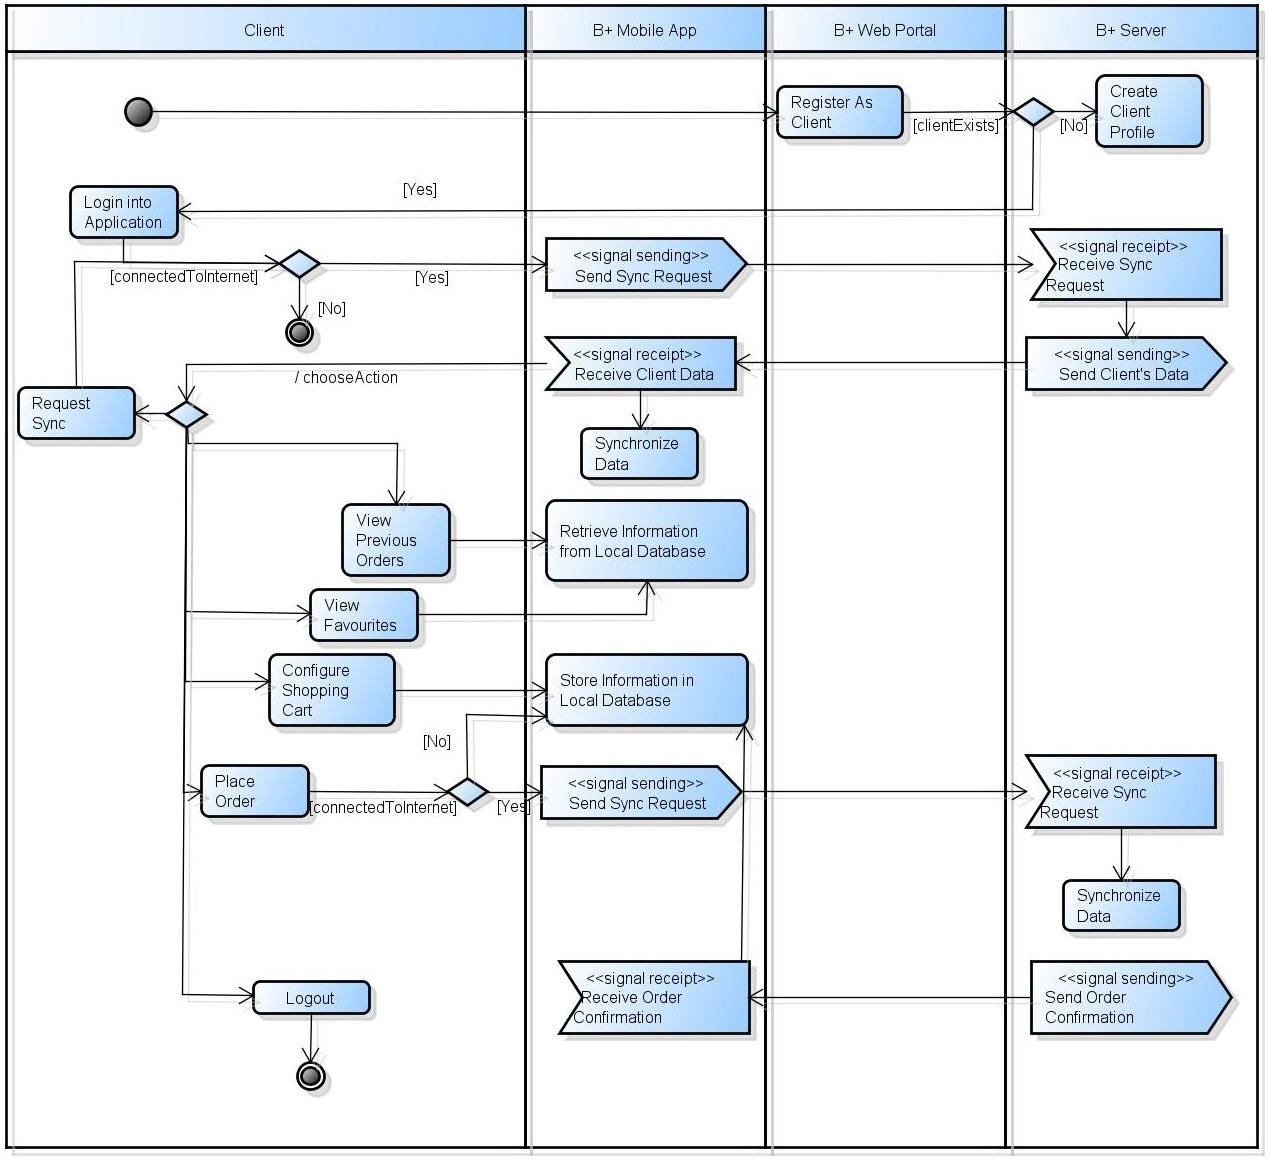
\includegraphics[scale=0.45]{Images/activity_diagram.png} 
%\caption[B+ Activity Diagram]{B+ Activity Diagram}
%\end{figure}
%\subsection{Business Perspective}
%\label{BusinesPerspective}
%\indent In order to better understand what functionality and what aspects an application must fulfill, it is important to understand and identify the goals of the application in the real environment. As the functions performed by the system can be analyzed only in correlation with its interaction with the users, it is important to capture these interactions. Stakeholders accomplish certain roles in the boundaries of an application and the most important parts of their interaction is captured in the use case diagrams. \\
%\indent Identifying the goals of the application in the context of real world interaction is important in defining the system functionality from a business point of view. Stakeholders fulfill certain roles in the processes involved in the program, and often their mission is captured in the use cases. Use cases illustrate a list of steps defining interactions between the system and a role with the purpose of the meeting a goal.
%\begin{figure}[ht]
%\centering
%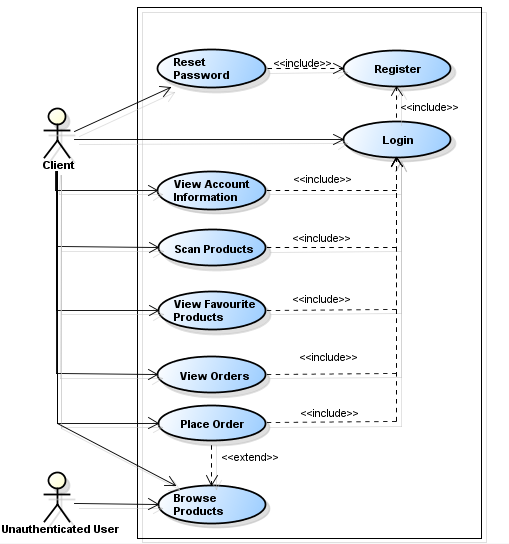
\includegraphics[scale=0.85]{Images/BusinessUseCaseDiagram.png} 
%\caption[Main Business Use Cases]{Main Business Use Cases}
%\end{figure}
%\section{Requirements Elicitation}
%\label{sec:Requirements Elicitation}
%\indent Being addressed to mobile devices, the system has to be aware of the existing limitations and has to be designed in such way it overcomes them. Due to the fact that connectivity might be restricted and intermittent, the amount of data transferred in a single step must be reduced as much as possible.\footnote{we are discussing now about the progressive synchronization and not the initial snapshot synchronization when the entire database must be replicated on the client side.}\\
%\indent As offline working mode is supported, users can perform many updates in the database while they are disconnected from the server. However, all of the changes executed in offline mode have to be synchronized with the server as soon as the user is connected.\\
%\indent Exchanging information is done in a standardized manner by using well - known data protocols. The most used protocols are XML and JSON, but between the two JSON is more flexible and is more easy to integrate with object oriented structures and relational data. Therefore, in B+, communication between the client side and the server side is done via JSON. We will describe more details about the JSON files with which the application works in the part dedicated to the communication between the client application and the server.\\
%\indent Computational resources required by the synchronization mechanisms should be reduced as much as possible. However, the server side was not adjustable and a big part of the computations had to be carried on at the client's side, reason for which the algorithm must be as efficient as possible.\\
%\indent Having an idea of the general restrictions that apply for the application, we will take a deeper look now at the functional and non-functional requirements.
%\subsection{Functional Requirements}
%\label{Functional Requirements}
%\indent The mobile application extends a part of the functions fulfilled by the B+ web portal. However, the focus is more oriented towards the ordering process and the offline working mode. 
%\begin{itemize}
%	\item \textbf{Account Management}. The application must allow the user to manage his account and authenticate himself in the application. Without authentication, the user must be not allowed to access the full functionality. The application must allow the user to view the information according to the customer they choose. This applies for both product information and customer information. Moreover, the user must be allowed to change some settings that will make his interaction with the application more intuitive.\\
%	\item \textbf{Content Coherence}. The application must keep the local database in a consistent state with the global database. Therefore, the information viewed on the mobile application must be consistent with the one that can be visualized on the web portal. Being aware of the fact that the system must also work in offline mode, it is important for it to mark and display distinctively the unsynchronized items to the users.
%	\item \textbf{Offline Working Mode}. The application must permit the user to continue his work in offline mode whenever no Internet connection is available. The transition from online to offline working mode must be signaled to the user in the case he wants to perform an action that is strictly dependent on Internet (first log in operation in the system, submitting an order to the server, requesting database synchronization).
%	\item \textbf{Component Communication}. Relying on different components, it is important for the application that the communication between them is properly established and functional. 
%	\item \textbf{History Retrieval}. Learning from user habits and extracting information from the past can be relevant for the user in deciding his further action or changing his behavior. The application must be able to query the data from the local database from user's past actions (user's favorite items, user's past orders). This information can be significant for the user for both speeding up the future ordering process by checking his favorite products or for building statistics by checking his previous orders.
%	\item \textbf{Alternative Input Methods}. Benefiting of specific hardware components, the application must allow the user to choose between different input methods when searching for specific products. The products can be retrieved either by searching after key fields, or by speaking this key fields using the speech-to-text functionality, or by scanning the barcode or another article possessed by the user. As speech-to-text input method is strictly dependent in this case on the performance of the built-in library on Android operating system, the application cannot guarantee a certain degree of reliability.
%	\item \textbf{Information Reuse}. Part of the information from the application that belongs to organizational details can be reused as input for other functions of the mobile phone. Phone numbers can be inputted directly in the phone's dialer, email addresses can be inputted as recipients for the email clients, links can be directed opened in browser for navigation. 
%\end{itemize}
%\subsection{Non-functional Requirements}
%\label{Non-functionalRequirements}
%\indent The following section analyzes the attributes of the system as a whole that define its quality.
%\begin{itemize}
%	\item \textbf{Security}. Every system handling private information should enforce security measures. User's information is kept under the privacy policy established in agreement with the company. Moreover, access to information is granted only after the authentication process is complete. The communication with the server is granted if the access token corresponding to the user is sent. Requesting the data from the server side is done under HTTPS communication either by GET or POST requests. GET requests are sent when general information is demanded, while private information is requested via POST requests.
%	\item \textbf{Usability}. The application is addressed to all users, regardless of their technical background or previous experience with mobile devices. The information flow and the commands must be easy to follow and straight-forward. The GUI must respect design principles that will enable the user to have an efficient interaction with the application.
%	\item \textbf{Performance}. Most of the use cases of the application are relying on the information stored in the database. A first improvement is replicating the data in a local database. However, in case of a database containing a large number of records, it is important to effectuate the queries in a restricted time range. The upper limit accepted for a query is 1 second. Synchronization operations are also time consuming and due to the fact that they are strictly dependent on the internet connection we cannot impose a certain time upper limit.
%	\item \textbf{Safety}. Mobile devices are power limited and might be run out of battery in the middle of a database operation. In case the device is turned off, data loss or data degradation must be avoided. The use of database transactions is desirable as they can roll back to the previous consistent state in the case of unexpected crash of the device or of one of the components.\cite{Transaction2004}
%	\item \textbf{Reliability}. The system must be up and running continuously without any problems. The dependence on the server side is cut by the offline working mode so any maintenance issues on the server side should not interrupt the client application of functioning normally.
%	\item \textbf{Robustness}. Working with client information, the application must be able to prevent any damage that can occur to it. The data of the application is stored at two sides: on both client and server side. In case any of the two fails, there exists the possibility to replicate the data from the other side. Also, important attention must be given to the communication components as some of the important problems that can alter the data happen during the communication between system components. There are cases in which the user can transform the data improperly by inputting or performing the wrong commands. We have tried to prevent this type of errors by providing him an intuitive interface that has its specific restrictions.
%	\item \textbf{Extensibility}. As business models evolve continuously and the type of information that has to be processed may vary, it is important to design the components of the system in such way they can be easily extended in the future. The database model can be easily extended by new tables with generic column types, the communication protocol can be varied according to the server exhibited API. Data exchange type can vary, reason for which the data exchange files and their parsers should be transformed without much additional effort.
%\end{itemize} 
%\indent All the previously mentioned non-functional requirements stand at the basis of the quality of B+ mobile application. Together with the functional requirements they define the guidelines for the design and the development of the application.
%\section{Database Component Structure}
%\label{sec:DatabaseComponentStructure}
%\indent B+ mobile application will work with a replicated, reduced version of the global database. The local copy will contain only the relevant information for the proposed use cases and even though the database schema will be the same on every device, the database entries will vary from device to device. The local database will contain only the information corresponding to the user(s) that have been logged in on the device.
%The database component of the application is built based on the SQLite database library provided directly by Android OS. In order to make it extensible and adjustable to new structure changes that the database can suffer, this component will contain interfaces and abstract classes that can be inherited correspondingly. We will structure our discussion in this chapter firstly on how the software part for the database is implemented, and in the end we will present the concrete database structure and the relationships among the tables.
%\subsection{Database Entity Relationship Diagram}
%\indent The following diagram reveals the structure of the physical SQLite Database stored in the mobile device. The local replica contains only a part from the global database that is needed for accomplishing the use cases earlier presented. The structure is built in a strong correlation with the business domain model of the mobile application and contains the main entities. By maintaining this local database the dependency on the global database and therefore, an internet connection is noticeably reduced.
%\label{subsec:DatabaseERD}
%\begin{figure}[ht]
%\centering
%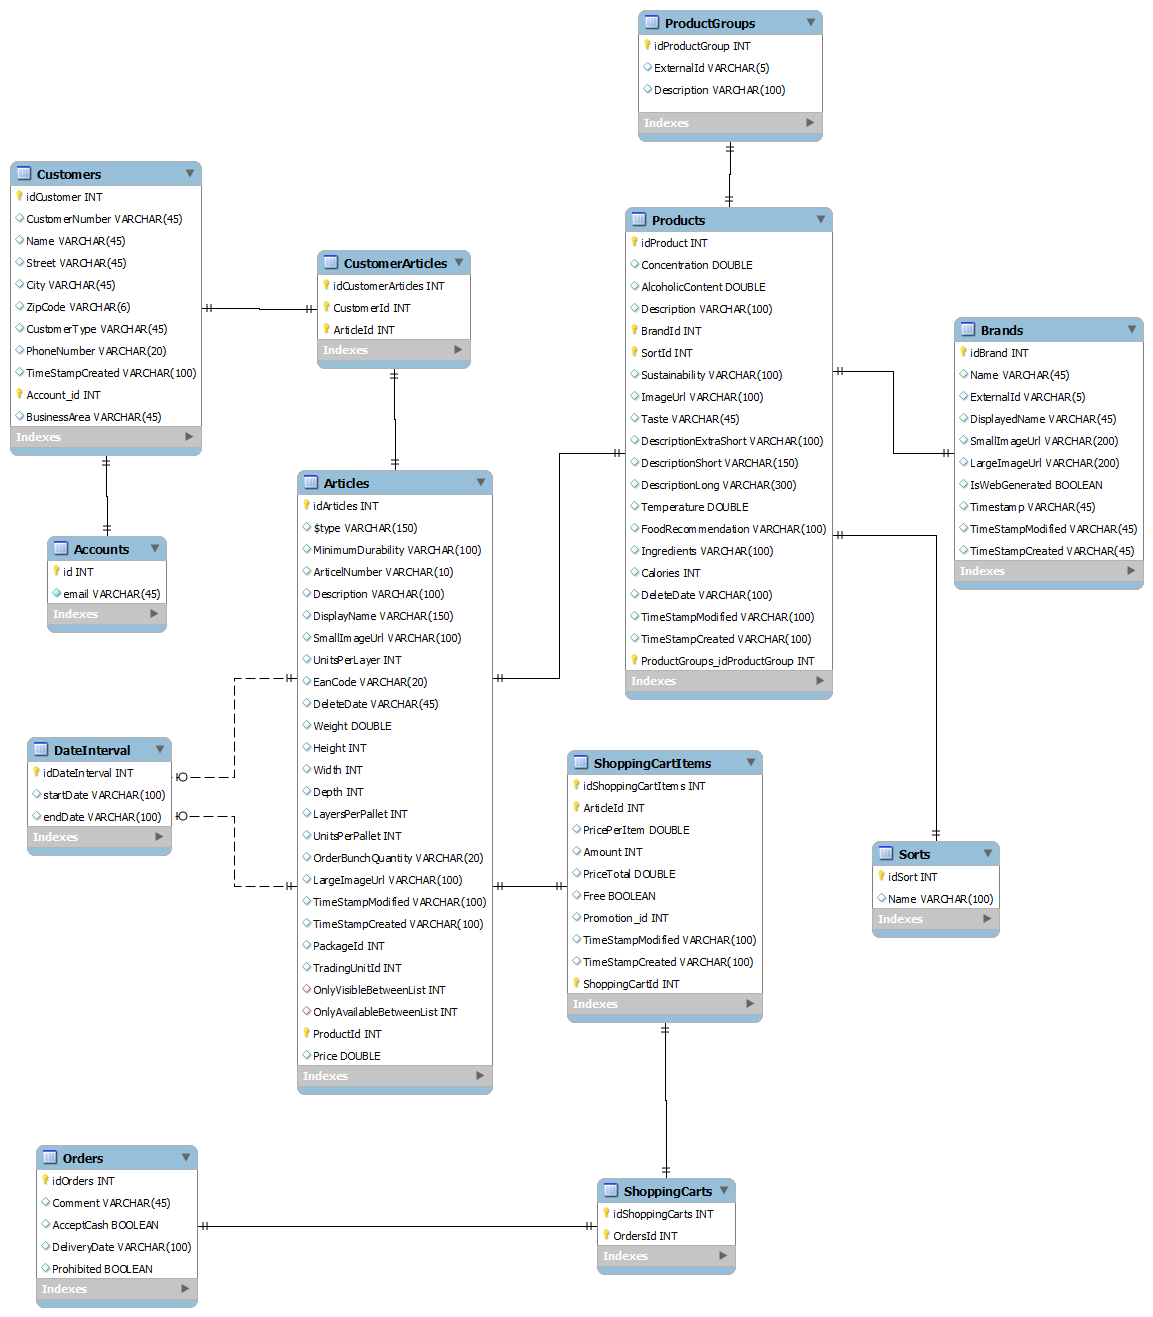
\includegraphics[scale=0.35]{Images/database_model.png} 
%\caption[Database Structure]{Database Structure}
%\end{figure}
%\subsection{Database Software Components}
%\indent The following section presents the main components needed for working with the database. This includes the object model classes corresponding to the tables of the database, the utility classes for querying and handling database instances. An optimization that can be brought to the operations performed with the database is mentioned at the end in the last part of this section.
%\label{subsec:DatabaseSoftwareComponents}
%\subsubsection{Database Model Classes}
%\label{subsubsec:DatabaseModelClasses}
%\indent Every physical table from the database represents a record of a certain type of entity. In order to work easier with the database entries, correspondents should be created in the software program. Intuitively, every table from the database has as equivalent a class, while every record of the table can be represented as an instance of that class. Knowing the database structure, the equivalent classes are built. The columns of the tables (name and type) will give the name and type of the attributes of the class. Another aspect we have to take into account when we create this classes is that they are a connection between the database and the rest of the application that works with database records. More specifically, whenever a piece of data from the database is needed in the program, it will be first represented as its corresponded class instance and then processed. The layer containing the database model is used also for building the serializable objects that are either received or sent with the JSON file exchanged with the server side.\\
%\indent In order to support further database extensions easier, this layer contains abstract classes for rows and generic column types. The abstract classes for rows are inherited by the actual database model classes, while generic column type contain attributes that define the traditional properties of database columns (primary key, foreign key, accepts null values).
%\subsubsection{Database Utility Classes}
%\label{subsubsec:DatabaseUtilityClasses}
%\indent One of the most important part of this layer handles the connection to the database and the creation and deletion of the database. This class extends the predefined SQLite Database Handler and is responsible with managing possible upgrades and downgrades of the database, performing given queries on the database, providing the necessary access and closing the connections that are no longer needed.\\
%\indent The database handler is the main manager of all the actions that are executed upon the database. As it is desirable to have only one instance that will coordinate these actions, we design this class as being a Singleton, therefore containing only one member that can be accessed by other classes.\\
%\indent The physical database will have no importance without the query operations that can be performed on it. From the insertions of the database records at the first synchronization with the server side, to different selections of data that is relevant for the user, the database queries are the mechanisms that provide the actual content displayed in the GUI. In order to retrieve and manipulate the data from the database, a query class has been created. This class is responsible with building the queries, and either persist the model objects in the database or create objects from the database entries. The queries are passed to the database handler which applies them on the working database. As resources are limited on the phone and fast data retrieval is important, these queries have to be created in an optimal way. We will talk more about optimizing the database component at the end of this subchapter.\\
%\indent Android SQLite Database library supports the management of different database versions by either upgrading or downgrading them. Management operations are essential as the database should suffer modifications according to some specific events. This aspect is important due to the fact that the local replica of the database keeps only relevant information for the active user. There are cases in which, the device can be used for several accounts and the database entries should be updated accordingly. As every customer has some specific articles and products that he can order, the local replica of the database should store only these records. On every user log out, the database should drop the tables that are user specific and need not to be persisted independent of the user session. On the other side, not all the information can be stored on the server side because the imposed restrictions. This information is relevant for the customer (details related to previously placed order from the device, favorite articles) and must not be deleted on user log out as he might want to access it in another session. Therefore, on the database upgrade and downgrade, only a part of the tables will be dropped.
%\subsubsection{Database Optimization}
%\label{subsubsec:DatabaseOptimization}
%\indent SQLite is a lightweight software library for SQL language that can be tailored for different platforms. Due to its characteristics it has been successfully used for numerous mobile applications. Android OS supports the use of SQLite databases by providing the libraries for managing private databases. B+ application will request data from the central database and create a local replica on the mobile device that will enforce offline working and faster data retrieval and processing. \\
%\indent The local replica saved on the mobile device stores only the data corresponding to the user(s) that are logged in on the device, reducing in this way the size of the database and the retrieval time of the information. Normal queries performed on databases have to be firstly compiled into byte - code program and then interpreted. The compilation step requires a considerable time and might be avoided if we keep into account the following observation. A query consists of a static part where normal SQL components (keywords) are included and a dynamic part that defines the properties of the database entries that should match the query. The static part repeats at every query request and its re-compilation can be avoided in order to reduce its processing time. Let us take the following example from B+ Application:
%\lstset{language=SQL,
%	keywordstyle=\color{blue}, 
%	xleftmargin = 0.5em,
%	xrightmargin = 0.5em,
%	keepspaces=true}  
%\begin{lstlisting}[breaklines=true]
%INSERT INTO Product (Id, Concentration, AlcoholicContent, Description, BrandId, SortId, ImageUrl, Taste, DescriptionExtraShort, DescriptionShort, DescriptionLong, Temperature, FoodRecommendation, Sustainability, Ingredients, Calories, DeleteDate, ProductGroupId,TimeStampModified, TimeStampCreated) VALUES (?, ?, ?, ?, ?, ?, ?, ?, ?, ?, ?, ?, ?, ?, ?, ?, ?, ?, ?, ?)
%\end{lstlisting}
%\indent This query handles the insertion of products in the local database. In the first synchronization of data, the number of product entries that need to be stored reaches the order of hundreds or thousands. Instead of compiling both the static and dynamic part for every entry, it is more efficient to compile only once the static part of the query and bind the dynamic part to every instance that needs to be stored. In our case the values that we need to store for different entries will be passed as binding parameters for the dynamic part of the query. Given a list of products that have to be stored in the database, we will iterate through this list, and bind the attributes of the product object with the parameters of the query, store the instance, and then unbind the parameters.\\
%\indent The dynamic part of the query corresponds to the attributes of the product that needs to be stored in the database. In order to optimize the querying process, the static part of the query can be precompiled, and re-used every time this query is requested. Precompiled statements have registered noticeable performances in comparison with normal queries.\\
%\indent B+ application works with data that has to be first captured from the global database and stored to its local replica and further on synced at periodical time intervals. The amount of data that has to be saved in the local database might reach the order of thousand of entries. A better approach is to perform the intended database operation for all the entries. This solution makes use of database transactions and also enforces data integrity as the operation can be either successful or failed.\cite{Hadzilacos1991} In both of this cases we know the exact state in which the database is. In the case of performing operations entry - by - entry, it is harder to detect where the process has been interrupted and from where it should be resumed. Database transactions are efficient for both batch row database operations and for ensuring that the database is in a secure state.
%\subsection{Database Persistence}
%\label{DatabasePersistence}
%\indent Information related to user's activity on the mobile device cannot be stored on the server side. The might like to check his history after a future authentication. Due to this aspect, this information must be persisted even after the user has log out from the application.\\
%The article catalog contains all the information related to products, brands that correspond to one user. On every log out action, the part of the database content related to the article catalog is deleted. These tables are re-created and the information is inserted on user's authentication. Log out action does not affect the tables that contain information about user's favorites, previous orders and shopping carts.\\
%\indent The favorite articles and previous shopping carts of one customer are resources  that can be used for speeding up the ordering process. This observation was drawn upon the activity of users on the web portal. Is has been noticed that every user has a certain range of products that he usually orders and the main parameters that vary are the quantities. On the mobile application, the user can check his history and create a new shopping cart based on a previous order. To this shopping cart he can add, remove or update items (modify their quantity).\\
%\indent While browsing through products, the user can mark an article as favorite and then retrieved it in the favorites screen. From the favorites screen, articles can be directly ordered. Keeping this information persistent over different sessions in the local database, the user can retrieve easily articles that are most likely to be ordered.\\ 
%\indent Article objects are the ones that can be entered directly in the order. Throughout application's life cycle they can pass through different states. The diagram from figure 4.4 illustrates the states in which an article object can be found. \\
%\begin{figure}[ht]
%\centering
%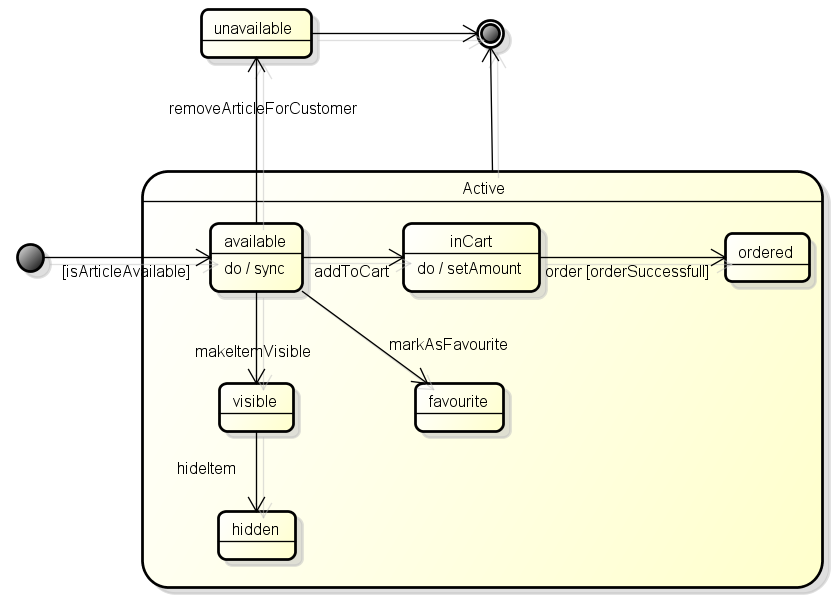
\includegraphics[scale=0.6]{Images/ArticleStatemachineDiagram.png} 
%\caption[Article Statemachine Diagram]{Article Statemachine Diagram}
%\end{figure}
%\indent Information about article catalog belonging to one user is subject to a periodical change and therefore, the corresponding tables will update their re cords after every synchronization process. The only permanent tables of the database are the ones for \textit{ShoppingCart, CartItem, Order}.
%\section{FileTransfer}
%\label{FileTransfer}
%\indent As the system focuses mostly on the ordering process, the graphical layout of the application implies also the transfer of files that come to the descriptive part of a product. In our case, the logos and the images that correspond to a product have to be loaded whenever the user reaches the section of the application. The images for brands come together with the application, while the images for products and articles need to be periodically synchronized as changes may occur on the server side.\\
%The request for pictures images receives as response a GSON archive. All the files of the archive are extracted using ZipInputStream and ZipEntry classes of Android and saved on the mobile device. Later on, they are directly loaded from the device.\\
%The synchronization of the data with the server includes both data and file synchronization. Files are changed rarely, reason for which they will be synchronized with a lower rate. 
%\section{Detailed Design}
%\label{sec:DetailedDesign}
%\indent The current section contains the technicalities of the mobile application. We will present the structure of the system and afterwards, analyze the its main components.
%\subsection{System Architecture}
%\label{Architecture}
%\indent B+ system is built in such a way that it allows both desktop users to access it via the web portal and mobile device users via the Android application. However, the operations that can be carried on are device specific and constrained somehow to the restrictions imposed by the hardware. It is significant to understand that the information in the global database can be retrieved and updated from both client application types and therefore it is essential to keep the local replicas of the database periodically synchronized on the mobile phones.
%\begin{figure}[ht]
%\centering
%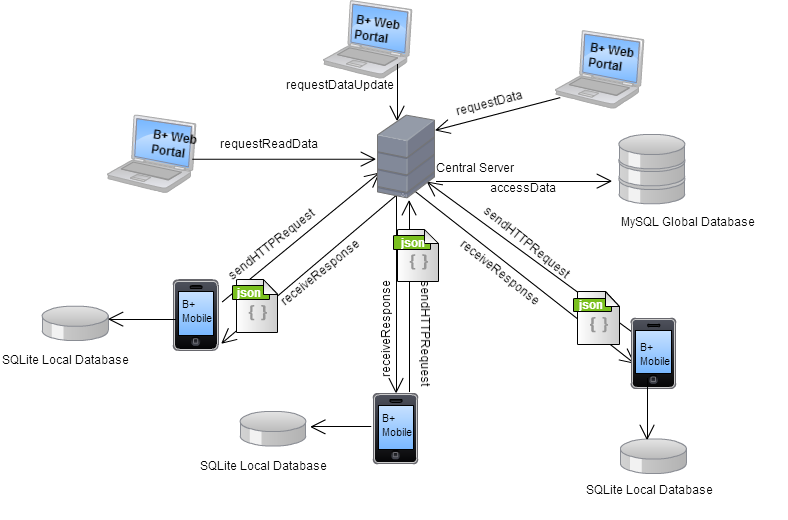
\includegraphics[scale=0.5]{Images/system_architecture.png} 
%\caption[System Architecture Diagram]{System Architecture Diagram}
%\end{figure}
%\indent Mobile applications send pull or push request either periodically or triggered by events. The communication with the server side is realized via HTTPS protocol and uses as message encryption language JSON. Pull requests are performed firstly on the first log in of the user and then periodically in order to keep the database information up-to-date. Push requests are more event oriented and are used to submit information about the orders placed by the users and their shopping carts. Normally, these requests should be carried on whenever the user completes the configuration of a shopping cart or places an order. However, due to the independence of an Internet connection this information is stored on the local database and pushed to the server when an Internet connection is available. 
%\subsection{Interfaces and Components}
%\label{subsec:InterfacesAndComponents}
%\indent Figure 4.5 exhibits the main components and interfaces of our mobile application. We will discuss them separately and their interaction in this section of the thesis. The components which rely on an external library will be presented in the next section of the thesis.
%\begin{figure}[ht]
%\centering
%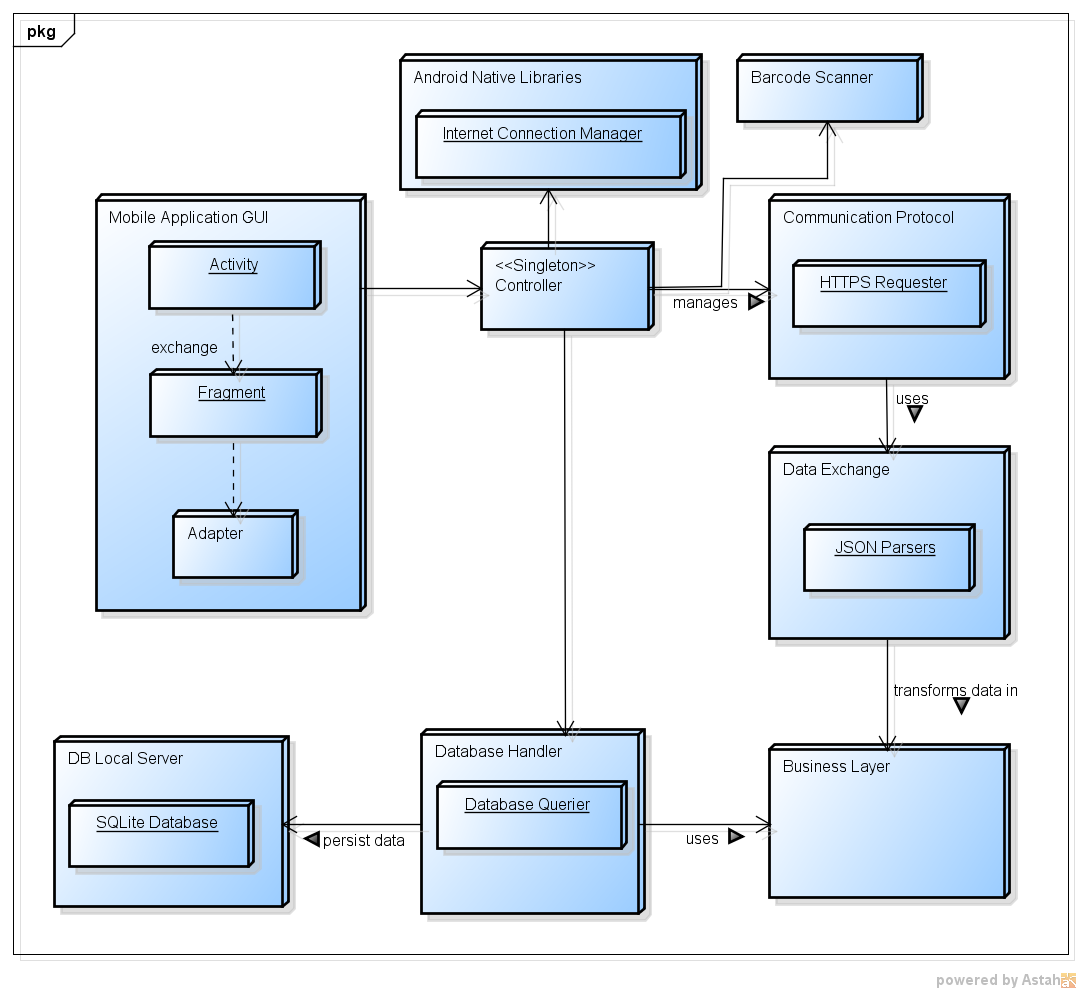
\includegraphics[scale=0.5]{Images/bplus.png} 
%\caption[B+ Components Diagram]{B+ Components Diagram}
%\end{figure}
%\indent The mobile application exposes an interface to communicate with the server API and exchange information. This interface is responsible with configuring the communication protocol and handling the authorization methods that need to be fulfilled. The communication with the server is based on HTTPS requests and responses. The requests from the server side can be either sent with the necessary parameters sent in the header or they can contain the meaningful information in a JSON file. We will present the sequence diagram for adding articles to the shopping part and placing orders in figure 4.6. This aims to illustrate the information flow in the application and way of interacting with the HTTP Client Service class that is responsible with the data exchange with the API.\\
%\begin{figure}[ht]
%\centering
%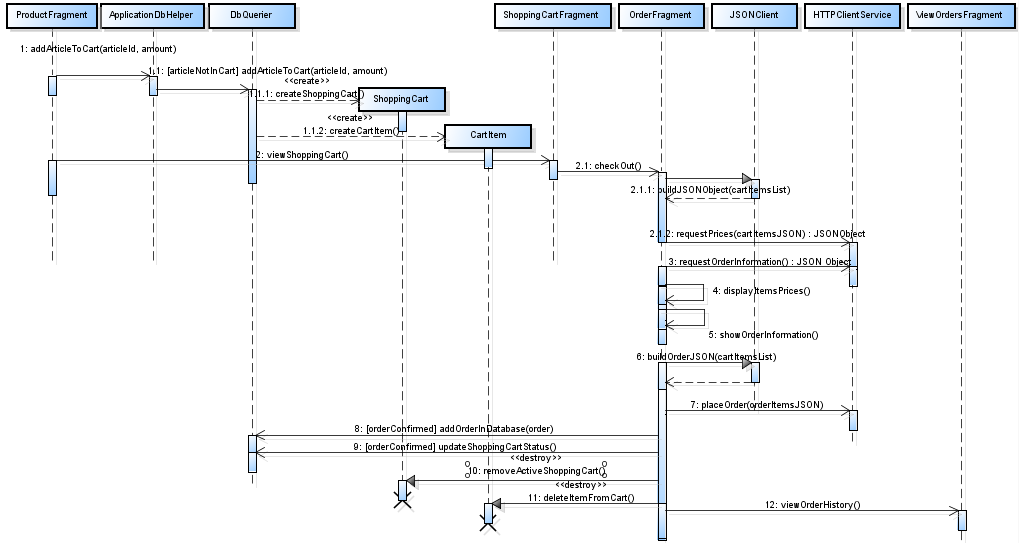
\includegraphics[scale=0.5]{Images/SequenceDiagram_placeOrder.png} 
%\caption[Order Placing Sequence Diagram]{Order Placing Sequence Diagram}
%\end{figure}
%\indent The GUI of the client application consists of Android Activities and Fragments that allow the user to perform different actions. After logging in into the application, the main activity just changes the fragments according to the request of the user. The use of fragments is important in loading information without the need of changing the layout. For example, inside the application, there exists the possibility to view different product categories or brands either as thumbnails (more graphical oriented by displaying the images) either as lists (compact view containing only the name). For the thumbnail view, the layout is the same but the actual content (image) differs depending on the navigation level at which the user is. For example, on the homepage (first navigation level) the user sees the product categories (as in figure 4.7, left side), while by choosing one of the product categories he will see the the brands belonging to the category (as in figure 4.7, right side). The whole process of changing from one level to another in fragments does not require reloading or rebuilding the layout. In this case, only the information with which the layout is filled is retrieved and displayed.
%\begin{figure}[ht]
%\centering
%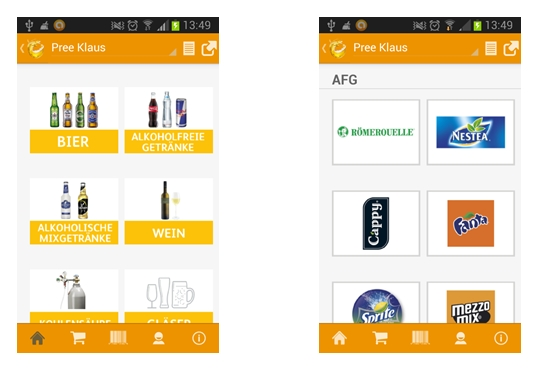
\includegraphics[scale=1]{Images/view_comparison.jpg} 
%\caption[Different Levels Fragment View]{Different Levels Fragment View}
%\end{figure}
%\indent The GUI is built in such way that it allows the user to easily navigate and retrieve the information he needs in as few steps as possible. The interaction that the user has with the GUI triggers different methods of the controller. The main application controller is a singleton class than handles all the logic behind the requests of the user from the GUI. It is responsible for calling the functionality of other components in an organized manner. We have chosen the design of this class as singleton due to the fact that we need only one instance to coordinate the requests. We will justify our choice by briefly presenting the singleton design pattern.\\
%\indent Singleton is a creational design pattern that allows the creation of only one instance of a class \cite{Gamma1995}. This instance can be accessed via a global point of access by other classes. The use of this design pattern is highly recommended for the classes that are responsible with the coordination of different processes or components. Our singleton class is responsible with handling the requests for the HTTP client, barcode scanner, and the transfer of data between the presentation and business layer of the application. This class is constructed in such way that the constructor is private, and its unique instance is accessed from a getter method. This method needs to call the private constructor in case the instance has not been created yet.\\
%\indent HTTP Client Service class is responsible with handling both GET and POST request and it also manages the request and response JSON information needed for the data exchange. The request JSON is formed before the method of this class is called and is given as a parameter, while the response file is received as a string from the server side and has to be parsed correspondingly. After receiving a response, the JSON client class is called given as parameter the response string. This class parses and transforms the JSON elements into meaningful objects with which the application can directly work (save them in the database, display them to the user, etc.).\\
%\indent JSON parser component works with GSON library that will be presented in the next chapter. It contains the necessary methods for interpreting and transforming JSON elements into their corresponding classes according to the type of information the JSON input contains. In order to be able to parse properly the contents of the JSON elements, it has to register all the necessary deserializers. Each deserializer is responsible with processing the fields of a certain JSON element and transforming it into its corresponding object. All the needed deserializers have to be registered before the JSON file is parsed.\\
%\indent Each deserializer contains the instructions or the rules to transform the fields of an element of the JSON input to attribute(s) of an object belonging to a certain class. They work directly with object model classes. JSON Parser component contains the JSON client class which is also responsible for transforming the objects into meaningful JSON elements. Saving the information about the objects into JSON files is needed whenever requests related to the shopping cart or the order placement are sent to the server. Usually, these requests contain the information about articles (article IDs, article amount in the shopping cart) needed either for providing the client side with the prices or with storing on the server side the needed information about the client's order. We have mentioned before the necessity of fetching the prices of the articles on demand whenever a checkout of the shopping cart is performed. The price field for articles is probably the field that suffers changes frequently. In order not to request synchronization every time a change occurs for the price field, the prices of the articles that are in the shopping cart are fetched from the server whenever the client checks out his shopping cart. This is the last step before filling in the order details and placing the order.\\
%\indent The object model classes are part of the business layer and they should comprise all the attributes that are relevant for the business process. Moreover, they correspond to the fields of the JSON elements and might contain additional information that is required to be stored in the local database (time stamp of the last synchronization, active/inactive elements). Because they could be used directly for serialization and deserialization of information for JSON files they implement the Serializable interface. This allows them to read or write instances from or to different I/O channels.\\
%\indent The object model classes are also the intermediary layer between the application and the information stored in the database. They are used inside the system in a bidirectional communication. Either the data retrieved from the database is stored in the form of objects and further on provided to the application, either the other parts of the application build objects that are then passed further to the DbQuerier class and stored as physical records in the database.\\
%\indent The Database Querier class handles all the incoming requests from the application with respect to saving, updating or retrieving information from the database. It works directly with the writable database instance of the SQLiteDbHelper and contains the method for building the queries and binding the parameters needed in the case of prepared statements. It also handles storing the retrieved information in object instances or collections of objects that are further on used by the application.\\
%\indent SQLite Database component is the local physical database, a cut-down replicated version of the global database. It stored all the information related to the authenticated user and the actions performed by him on the device. Due to the fact that the functionality provided by the server is limited, there are some tables that contain information which cannot be retrieved if the user logs in on another device. Such local data is related to favorite articles, or order placed from the mobile device. This data is relevant in case the user wants to customize the application, view its history and/or speed-up the ordering process.
%\subsection{Information Flow}
%\label{InformationFlow}
%\indent The sequence of steps executed by the user can lead to different outcomes. In this section, the main actions and screens that are available for one user are mentioned:
%\begin{itemize}
%	\item \textbf{Customer Information}. The user can easily exchange from one customer to another in case it has more customers associated to his account. Information related to his account can be retrieved on the account information menu and includes order history, favorite items and customer information. The most important screens containing customer information are illustrated in the figure 4.9.
%	\begin{figure}[ht]
%	\centering
%	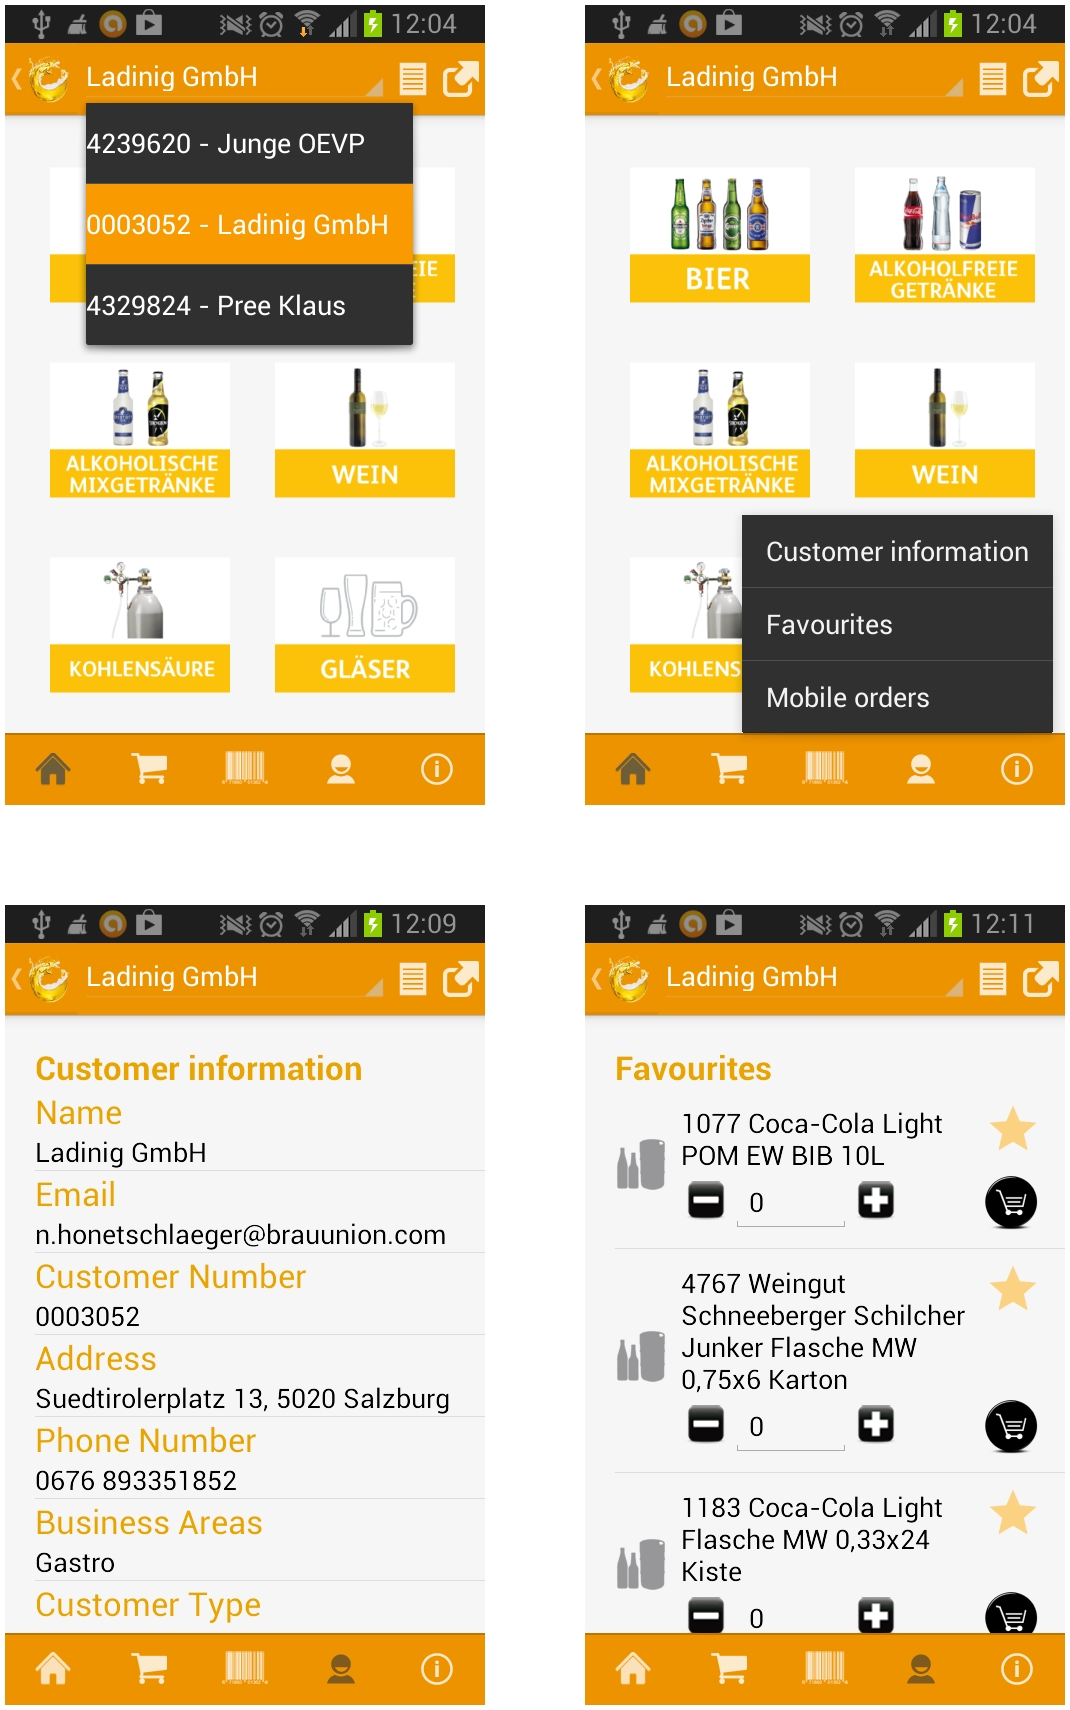
\includegraphics[scale=0.35]{Images/account_view.jpg} 
%	\caption[Customer Information Views]{Customer Information Views}
%	\end{figure}
%	\item \textbf{Application Information}. In order to preserve this part as similar as possible to the original portal, a WebView component has been used. In this part of the application, legal information, useful links and contact data is found. Figure 4.10 presents two views containing information related to the application.
%	\begin{figure}[ht]
%	\centering
%	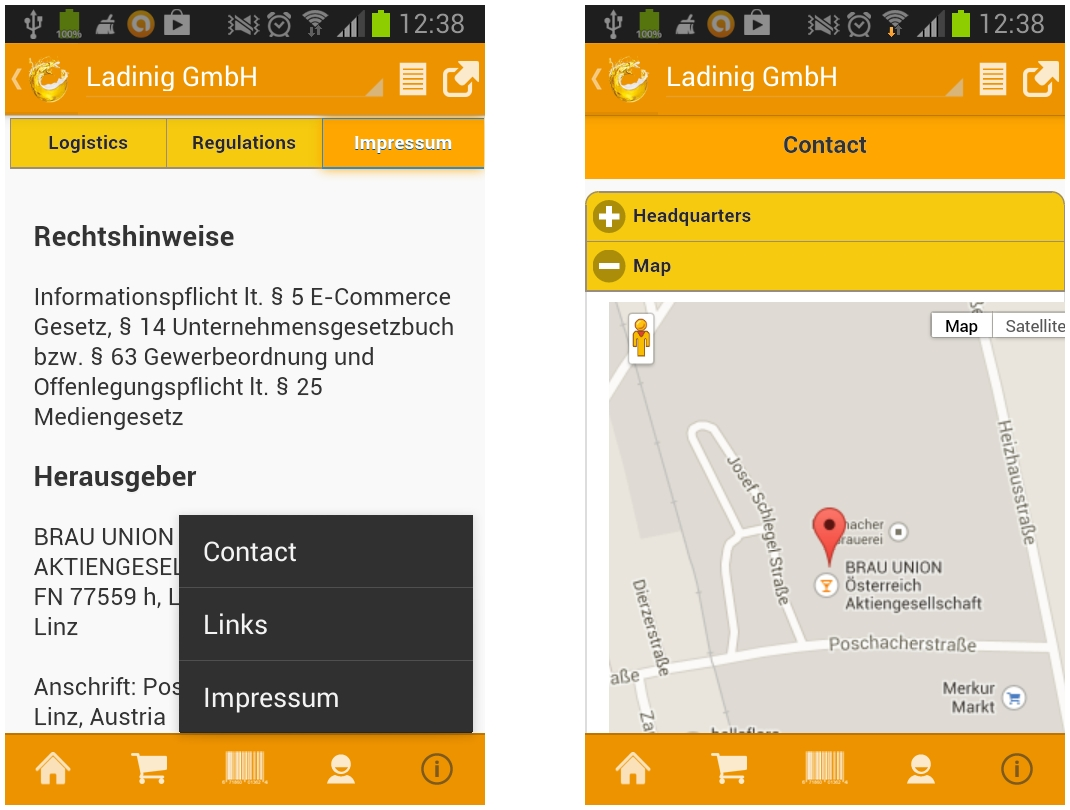
\includegraphics[scale=0.35]{Images/contact_view.jpg} 
%	\caption[Application Information Views]{Application Information Views}
%	\end{figure}
%	\item \textbf{Ordering Process}. The process of ordering involves choosing the article that should be added in the cart, viewing the shopping cart and checking out the order. After receiving the prices and defining the order details (address, date), the order is sent to the server. Details of the order can be further on retrieved in order history screen for the customer menu. In figure 4.11, some screens involved in the ordering process are displayed.
%	 \begin{figure}[ht]
%	\centering
%	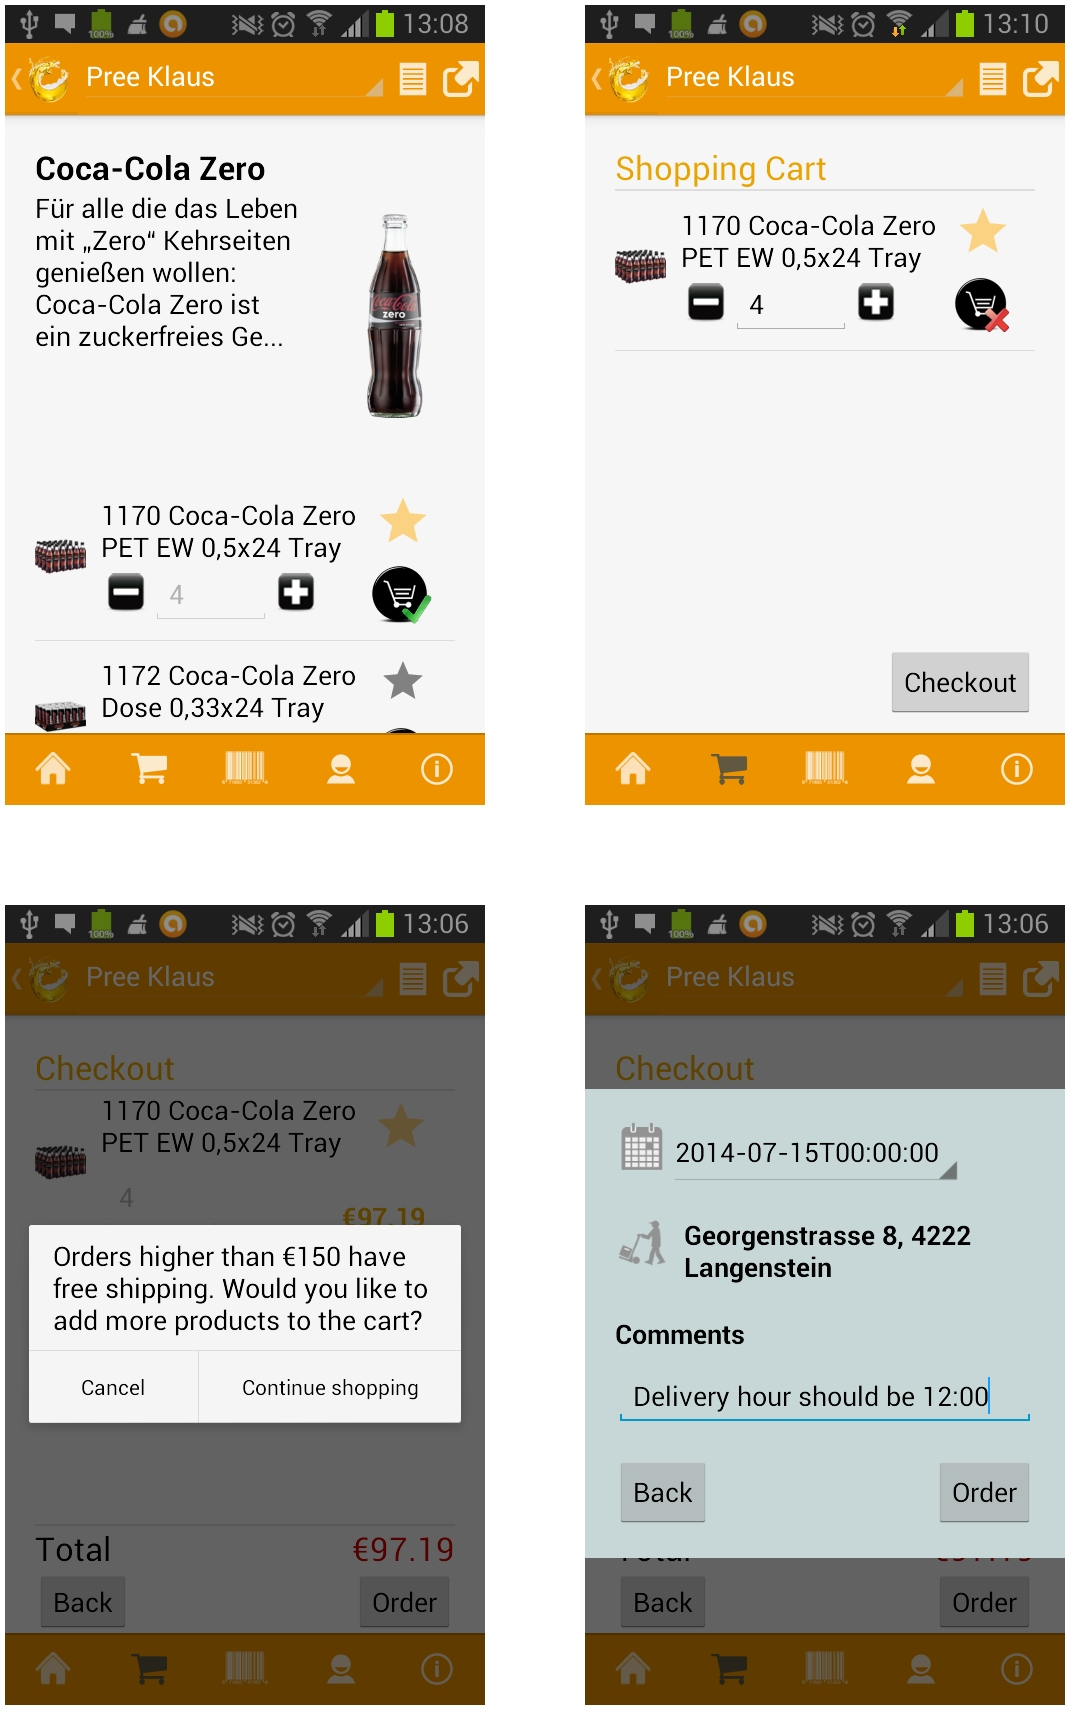
\includegraphics[scale=0.35]{Images/order_view.jpg} 
%	\caption[Application Information Views]{Application Information Views}
%	\end{figure}
%\end{itemize}
%\subsection{Background Synchronization}
%\label{Background Synchronzation}
%Besides the capture synchronization that occurs after user's authentication, periodic synchronization with the server must be performed. Data from the client side that needs to be sent to the server contains details about the shopping cart and the order. This data is pushed to the server whenever the device has a functional Internet connection. However, most of the changes related to the article catalog (brands, sorts, products and articles) occur on the server side. They should be pulled on a periodical basis.\\
%The periodical synchronization with the server side is performed in the background daily and is handled by a service so that the user does not need to trigger it. It includes the information stored in the database for the current user. Files are treated in a different manner and they are also synchronized with the server side but on a weekly basis.\\
%The synchronization method is listed in the following code.
%\subsection{External Dependencies}
%\label{ExternalDependencies}
%\subsubsection{JSON Parsing}
%\label{JSONParsing}
%\indent The exchange of information between the client and the server side relies on transmitting JSON files. These files contain meaningful information for the type of the data pushed or pulled. As the information exchanged can be extended or reduced in time depending to the business requirements, the schema and the structure of the JSON document is also subjected to change.\\
%\indent In order to work with the JSON document and extract the information into object instances or conversely transforming objects into structured JSON document, we have used a JSON library that is suitable for Android mobile applications, GSON\cite{Gson2014Library}. In comparison with other similar libraries, GSON focuses on providing the suitable methods for using generic objects or retrieving information without being required to use annotations.\\
%\indent One of the fundamental concepts behind GSON is reflection. Using reflection, a program is able to modify its structure and behavior at run-time. In this case, GSON can interpret at run-time how it should build the JSON file according with the domain classes or conversely how it should construct the objects knowing their attributes and the fields contained in the JSON file. In case of null values, the corresponding field is by default not initialized, but this exception can be handled differently if needed.\\
%\indent GSON is suitable for the case of software systems using collections, nested and inner classes and for which the data with which they work is susceptible to frequent changes. Normally, for every entity, it is necessary to write the class with the specific attributes and constructors and call the deserializer for the class. In case the information from the JSON files has to be written or read in a specific way, a particular deserializer for the corresponding class can be written.
%
%\subsubsection{Barcode Scanner Library}
%\label{BarcodeScanner}
%\indent Even though mobile devices have certain resource limitations, they can also provide users some functionality that cannot be found on normal computers. One of the examples sustaining this idea is the barcode scanning functionality. With the aid of mobile device camera, one can easily scan barcode and QR codes that can be later on used in the retrieval of certain products information. For B+ Android application, the barcode scanning function is one of the features that distinguish it from the web application. It also improves the user's experience by allowing multiple input methods. The main aim of implementing this functionality is to enhance the ordering process.\\
%\indent Android QR Response code is one of the extensions of ZXing barcode scanner library. It allows decoding information about different articles by processing their barcode image and obtaining their EAN code. This library comes with an integration module that allows third party applications to easily include it in their own work flow. In our case, a request for the scanner can be sent from the GUI. The GUI button has a listener which in its turn calls the controller. The controller is responsible for starting the scanning intent. In the scanner activity, the user can easily scan the barcode of his desired article. If the scanning process is complete and an article having a corresponding EAN code is stored in the device's database, the user is displayed a screen with the information of this article. Besides barcodes, this library is able to decode the information contained in QR codes.\\
%\indent Inside the application, the user can directly scan the barcode and retrieve its corresponding article (in case it exists). After retrieving the article, the user can view the product, added it to the shopping cart or mark it as a favorite. As one can notice, the main functionality of the barcode scanner is the easy retrieval of the product articles. Figure 4.9 illustrates the use of this function.
%\begin{figure}[ht]
%\centering
%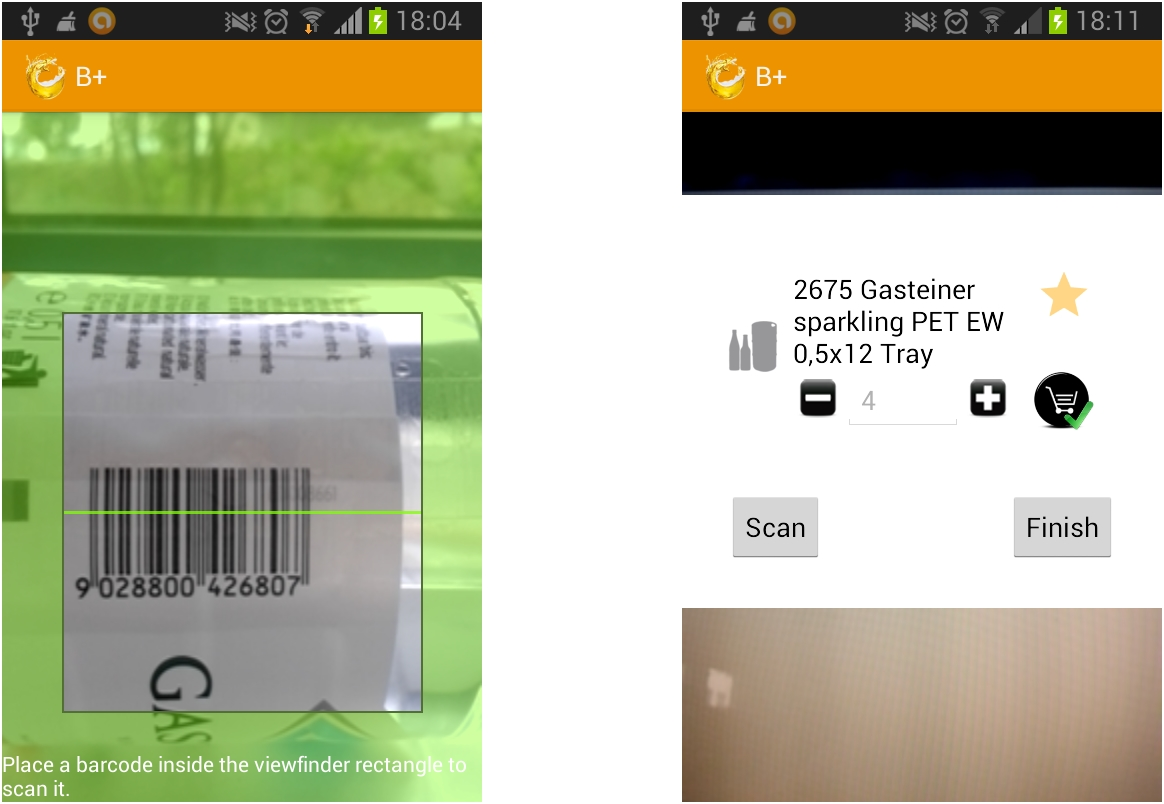
\includegraphics[scale=0.45]{Images/barcode_scanner.jpg} 
%\caption[Barcode Scanning Functionality]{Barcode Scanning Functionality}
%\end{figure}
%\subsubsection{WebView Component}
%\label{WebViewComponent}
%\indent Android applications can directly display web pages inside a graphical layout with the aid of WebView. The actual communication between Android client application and WebView is ensured via a Javascript interface. If the actual content is just for presentation there is no need to implement this interface.\\
%\index In our application, WebView is used for displaying useful information (contact data, frequently asked questions, contact links) in the form of a web page. By displaying this content in the form of a web page will make it more consistent with the web portal. However, using WebView is not desirable in the case of retrieving information from database and displaying it. This happens because interfaces built with HTML, CSS go hand in hand with Javascript which is an interpreted language. Interpreted languages are slower than compiled languages, therefore a web page inside a mobile application will be slower than a native application in which graphic elements are displayed via proprietary APIs and abstractions\cite{Charland2011}.
%\index All the graphical elements for the WebView component are built with jQuery mobile so that they are compatible and properly displayed independently of the device resolution or OS version. jQuery mobile library is a framework that allows developers to customize the web page elements, build transitions and effects and handle different types of events. In order to be able to interpret the Javascript functions, the activity that contains the WebView pages has to enable Javascript content. This is mostly required for the contact page that embeds a Google Map which is rendered with the aid of a Javascript function.\\
%\indent The advantage of WebView is that it allows navigation between specific parts of its content as easy as navigating a web page. For contact elements, it launches automatically other applications (e-mail client in the case of an e-mail address link, browser in the case of a link, dial pad in the case of a number).
%\subsubsection{Generation of PDF Documents}
%\label{PDF Documents}
%\indent Mainly, all of the information of the application is stored in the database and receives in this sense a physical form. However, some of the use cases of the application require the generation of files containing information from the database. For example, invoices of orders should be displayed to the user in a form close to the paper-written invoices. For this reason, the information comprised by them is included in a PDF document that can be either viewed or saved by the user on his device.\\
%\indent Libraries created for latest versions of Android OS support the generation of PDF documents in a similar way like adding graphical items to a canvas element. We are not able to use this approach as the aim was to make the application available also for older Android OS versions. This is the main reason behind choosing an external Java library for generating PDF documents.\\
%\textbf{PDFJet} is a lightweight library for both Java and .NET. Being lightweight and portable it covers the need of mobile applications running either on Android or Windows Phone OS. It allows the generation of PDF documents on which different graphical or text elements can be added. It is suitable for the presentation of data in different ways (tabular, written, graphical) and allows its creation in an object oriented manner.
%
%\section{Challenges}
%\label{sec:Challenges}
%\subsection{Portability Issues}
%\label{PortabilityIssues}
%\indent As already known, Android OS can be deployed on a large number of devices and has a non-standardized character. The OS has been changed among time in order to support newer graphical elements or to make it more ubiquitous by supporting more functions. However, some of the active devices are still running on older versions which do not support some of the new elements and this might cause compatibility problems. The purpose of the application was to allow as many customers as possible to make use of it. That was the reason for which we have decided to build the application for Android versions newer than Android Gingerbread(2.3.3). Because the most important changes on Android occurred on version higher than 3.0, some of the components that ensure the user interaction that are native could not be implemented.\\
%\indent An alternative to them is, however, offered by ActionBarSherlock library. It permits the use of elements like Action Bar, Fragments, Contextual Menu and it can be integrated for applications running on older Android OS versions. Despite the fact that it is a good replacement, there are still some components that it cannot perfectly reproduce. For instance, in the case of action bar menus that contain more elements than can be displayed in the layout, no overflow item is displayed. The consequence is that these elements simply disappear and are not available for the user.\\
%\indent We have used this library also for adding the navigation drawer component to the application. It should allow the user to easily navigate through the products and search products after some of their main attributes (name, description).\\
%\indent The result of using this library was the possibility to add more elements that can improve the user experience and make them available for different devices. The lack of standardization for Android OS is one of the main issues when designing the applications. The variety of device sizes, resolutions are a challenge for building consistent layouts and styles. Luckily, some of the existing libraries enforce the possibility to use newer elements on older versions.
%\subsection{Server Side Dependency}
%\label{ServerSideDependency}
%\indent The mobile application works with a replicated copy of a global database stored on the server side. The client application has to communicate periodically with the server side for exchanging information (either pushing or pulling data or both). Because the exchange of all data is not needed (usually, only a part of the information from the database is changed), it is important to perform the synchronization only for those items that suffered the change. It is preferably to keep the check of the items that require to be synced on the server side as it might consume resources that are more limited on the mobile device.\\
%\indent The problem with the B+ application is that it can only work with a given API from the server side. This API ensures the authentication of the user, authorization of performing certain actions, data exchange between the client and the server. The functions needed for executing these actions are called from the client side using HTTPS requests and are fixed.\\
%\indent In order to exchange data with the server, the user should be able to confirm his identity. After a successful authentication, the server sends to the client an access token that will be used for further operations. This access token is stored in device's SharedPreferences until the user logs out of the application. This information is private and can be retrieved only in the application context. In case the application is on a different screen than the log in or register ones and no access token is detected, the user will be redirected to the log in screen.\\
%\indent The token possessed by the user on his device is used in the authentication to get access to resources. The access is granted without the need of proving that the bearer possesses a cryptographic key. In order to keep it safe from other misuses, the token can be retrieve only from inside the application and is destroyed after the user logs out.\\
%\indent The connection to the server side API is realized by HTTP requests containing the bearer's access token. Requests contain the URL of the API function that provides the requested information, input parameters for the request (customer number, articles IDs) and the content type of the request.\\
%\indent Extending the server side functionality is not handled for our work, reason for which we are strictly dependent on the methods provided. This can constitute a problem whenever on the client side a new function that needs new data from the server side is built. At the current time, it allows data push and pull filtered according to the user, respectively the active customer. No filter for data that has suffered changes or it is not synchronized is handled. Because no checks for data synchronization can be performed on the server side, the information should be verified to be consistent on the client side.
%\section{Deployment and Installation}
%\subsection{Application's Permissions}
%\label{Application's Permissions}
%\indent Once installed on the device, the application requires some permissions to use other Android OS components. Most of the users are skeptical about applications that request many permissions, reason for which we tried to reduce them. Mainly, the application needs access to the following components:
%\begin{itemize}
%	\item \textbf{Camera}. This component is needed by the barcode scanning function of the application.
%	\item \textbf{Internet}. In order to communicate with the server side, the application needs an active Internet connection.
%	\item \textbf{Access Network and Wi-Fi state}. After data synchronization, the application can be used in offline mode, unless the user desires to send an order to the server. In case the user wants to place the order, the application must check if either a network (3G) or Wi-Fi Internet connection is active. If not, the order is kept in the local database until the device is successfully connected to the Internet.
%\end{itemize}
%\subsection{Installation}
%\label{Installation}
%\indent The application will be distributed to the user via Google Playstore platform. The users can directly download and install it without no further constraints. However, in order to get access to the application they need to have a valid account and at least a customer number previously created on the web portal.